\section{Thread}
Un thread è l'unità fondamentale della computazione, può essere generato da un processo aprendo la possibilità alla \textbf{parallelizzazione} della task.

\spacer
I thread appartenenti allo stesso processo condividono codice, dati e risorse (ad es. una modifica ad una variabile globale oppure l'apertura di un file sono visibili a tutti i thread)

Queste situazioni vanno però gestite correttamente, altrimenti si rischia di di avere conflitti nell'accesso alle risorse.

\begin{figure}[H]
    \centering
    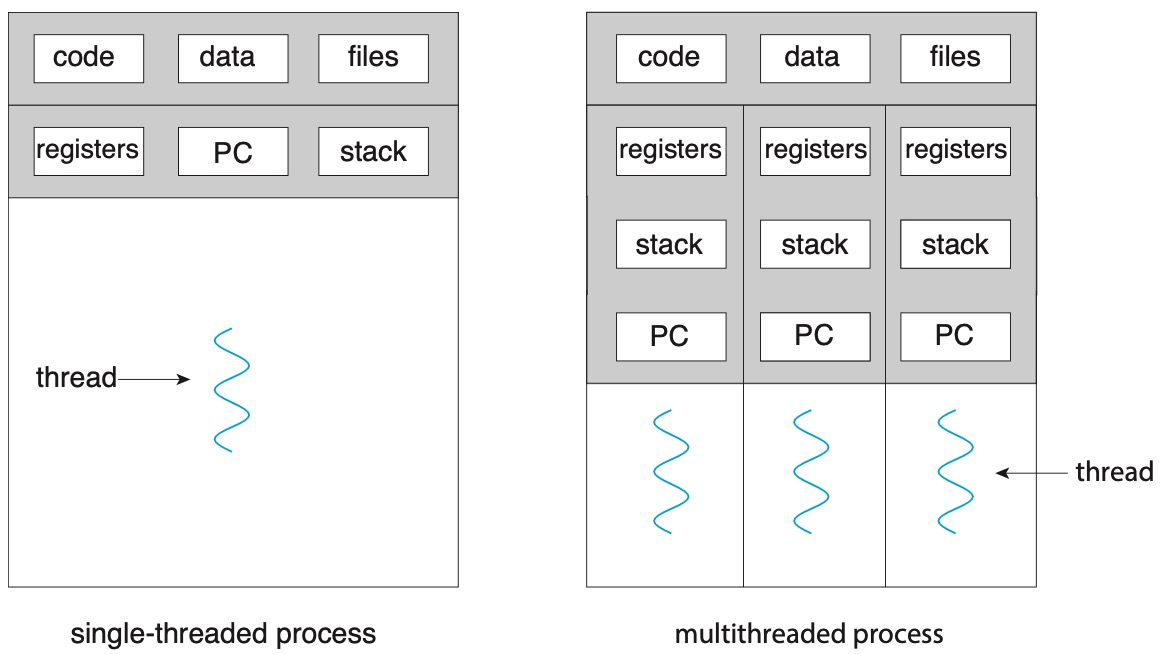
\includegraphics[width=0.6\linewidth]{assets/multithread.jpg}
\end{figure}

\spacer

Il thread comprende:
\begin{sitemize}
    \item un identificatore di thread
    \item un contatore di programma
    \item un insieme di registri
    \item uno stack
\end{sitemize}

\begin{note}
    Il processo tradizionale, che viene eseguito su un singolo processo, si definisce "\textit{heavyweight process}", mentre i thread sono detti anche "processi leggeri".

    \spacer[4pt]

    Un thread può essere utilizzato dal browser per rappresentare una singola pagina web, per generare velocemente icone per una serie di immagini oppure possono essere usati da un webserver, un thread per ogni richiesta.
\end{note}

\subsection{Visualizzazione}

Per visualizzare lo stato di un processo in relazione al tempo useremo dei grafici con il tempo sull'asse x, e lo stato del processo sull'asse y.

\begin{figure}[H]
    \centering
    \begin{minipage}{0.45\textwidth}
        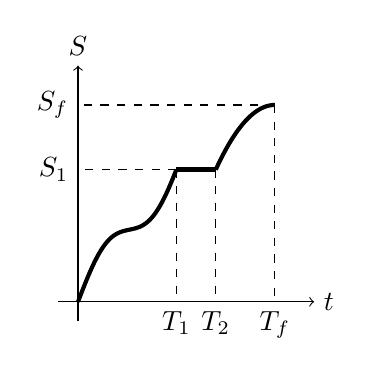
\begin{tikzpicture}[scale=2.5]
            % assi
            \draw[->] (-0.1,0) -- (1.2,0) node[right] {$t$};
            \draw[->] (0,-0.1) -- (0,1.2) node[above] {$S$};

            % funzioni
            \draw[domain=0:0.5,smooth,variable=\x, line width=1.5pt] plot ({\x},{1.4*\x+1/10*sin(deg(12*\x))});
            \draw[domain=0.5:0.7,smooth,variable=\x, line width=1.5pt] plot ({\x},{0.672});
            \draw[domain=0.7:1,smooth,variable=\x, line width=1.5pt] plot ({\x},{ -2.65 + 7.3*\x - 3.65*\x^2});

            % riferimenti
            \draw[dashed] (0.5,0.672) -- (0.5, 0)  node[below] {$T_1$};
            \draw[dashed] (0.7, 0.672) -- (0.7, 0) node[below] {$T_2$};
            \draw[dashed] (1, 1) -- (1, 0) node[below] {$T_f$};
            \draw[dashed] (0.5, 0.672) -- (0, 0.672) node[left] {$S_1$};
            \draw[dashed] (1, 1) -- (0, 1) node[left] {$S_f$};
        \end{tikzpicture}

        In questo caso particolare si può notare un periodo di tempo, da $T_1$ a $T_2$ dove il processo rimane nello stato $S_1$, questo indica che si trovava in un \textit{bottleneck}, ovvero il processo stava attendendo una qualche risorsa.
    \end{minipage}
    \hfill
    \begin{minipage}{0.45\textwidth}
        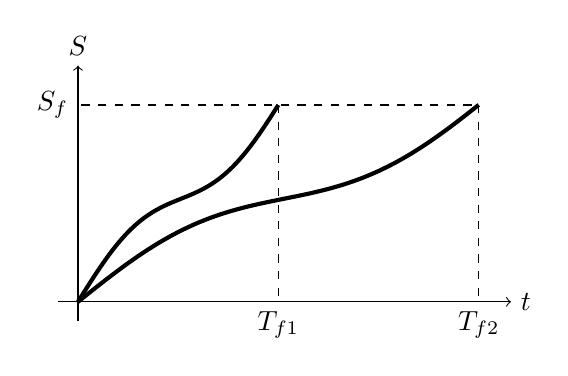
\begin{tikzpicture}[scale=2.5]
            % assi
            \draw[->] (-0.1,0) -- (2.2,0) node[right] {$t$};
            \draw[->] (0,-0.1) -- (0,1.2) node[above] {$S$};

            % funzioni
            \draw[domain=0:1.018,smooth,variable=\x, line width=1.5pt] plot ({\x},{\x+1/10*sin(deg(6*\x))});
            \draw[domain=0:2.036,smooth,variable=\x, line width=1.5pt] plot ({\x},{0.5*\x+1/10*sin(deg(3*\x))});

            % riferimenti
            \draw[dashed] (1.018, 1) -- (1.018, 0) node[below] {$T_{f1}$};
            \draw[dashed] (2.036, 1) -- (2.036, 0) node[below] {$T_{f2}$};
            \draw[dashed] (2, 1) -- (0, 1) node[left] {$S_f$};
        \end{tikzpicture}

        In questo casolo stesso processo viene eseguito su due processori diversi, $T_{f1}$ è il processore più veloce, mentre $T_{f2}$ quello più lento.
    \end{minipage}
\end{figure}

\subsection{User e Kernel Threads}
Nei moderni sistemi operativi esistono threads al livello utente e altri al livello kernel.
Quando un thread a livello utente fa una chiamata a sistema è necessario trovare un thread a livello kernel che sia pronto ad accettarla, altrimenti si rischia di introdurre dei tempi di attesa.
Va quindi trovata una relazione tra le due tipologie di threads.

\subsubsection{One-to-One}
Mappa ogni thread a livello utente con un suo corrispettivo a livello kernel, questo assicura che ogni \textit{systemcall} venga gestita correttamente e rapidamente.
Tuttavia così facendo si creano molti thread che potrebbero portare ad una riduzione delle prestazioni.

\begin{figure}[H]
    \centering
    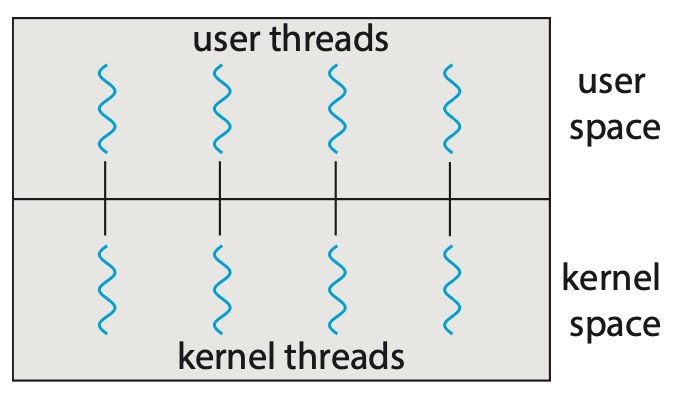
\includegraphics[width=0.35\linewidth]{assets/one-to-one.jpg}
\end{figure}

\subsubsection{Many-to-Many}
Questo modello mappa $n$ thread utente a $k$ thread kernel, dove $n << k$. Questo modello ha una migliore utilizzazione delle risorse, ma è di difficile realizzazione la funzione che associa thread utente a thread kernel.
Ad oggi nessun sistema operativo moderno lo utilizza, si preferisce usare il modello one-to-one.

\begin{figure}[H]
    \centering
    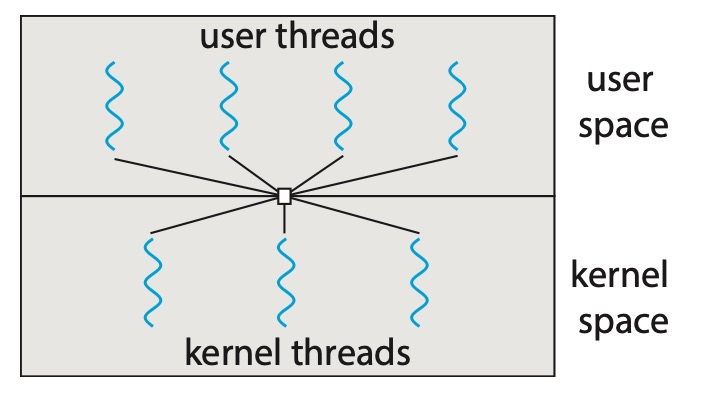
\includegraphics[width=0.35\linewidth]{assets/many-to-many.jpg}
\end{figure}

\subsection{Implementazioni}
\subsubsection{Linux}
Linux implementa la Process Control Block mediante una \textit{task struct}, la ready queue diventa quindi una lista concatenata di \textit{task struct}.

\spacer
Quando un processo crea uno o più figli può scegliere se continuare la sua esecuzione in parallelo con essi o se attendere la loro conclusione.

Inoltre può scegliere se eseguire lo stesso codice del genitore o un altro programma.

\spacer
In linux, come in molti altri Sistemi Operativi, tutti i processi sono figli di un processo iniziale, nel caso di linux è il processo con ProcessID = 1.

Un nuovo processo viene generato con la funzione texttt{fork()} che restituisce l'id del nuovo processo al parent e restituisce 0 al figlio, questo è importante perché permettere di distinguere se ci si trova nel parent o nel children.

Quando il genitore non attende l'esecuzione dei figli e termina prima di essi essi sono detti \textbf{orfani} e alla loro terminazione diventano degli \textbf{zombie}.

\subsubsection{iOS}
Nelle prime versioni era previsto un solo processo utente in esecuzione.

A partire da iOS 4 vengono permessi anche dei processi di background, a priorità inferiore rispetto a quello di foregorund che ha il controllo della GUI.

\subsubsection{Android}
Le applicazioni che vogliono continuare l'esecuzione in background devono utilizzare un servizio.

\spacer
Quando dei processi devono essere terminati la selezione avviene secondo l'ordine:

processi vuoti -> background (non evidente all'utente) -> di servizio (evidente all'utente) -> visibile (usati da un processo foregorund) -> foregorund.

\subsubsection{Chrome}
Google chrome usa un processo di gestione del browser, dell'interfaccia utente, dell'I/O, poi utilizza un processo renderer per ogni pagina di navigazione.
